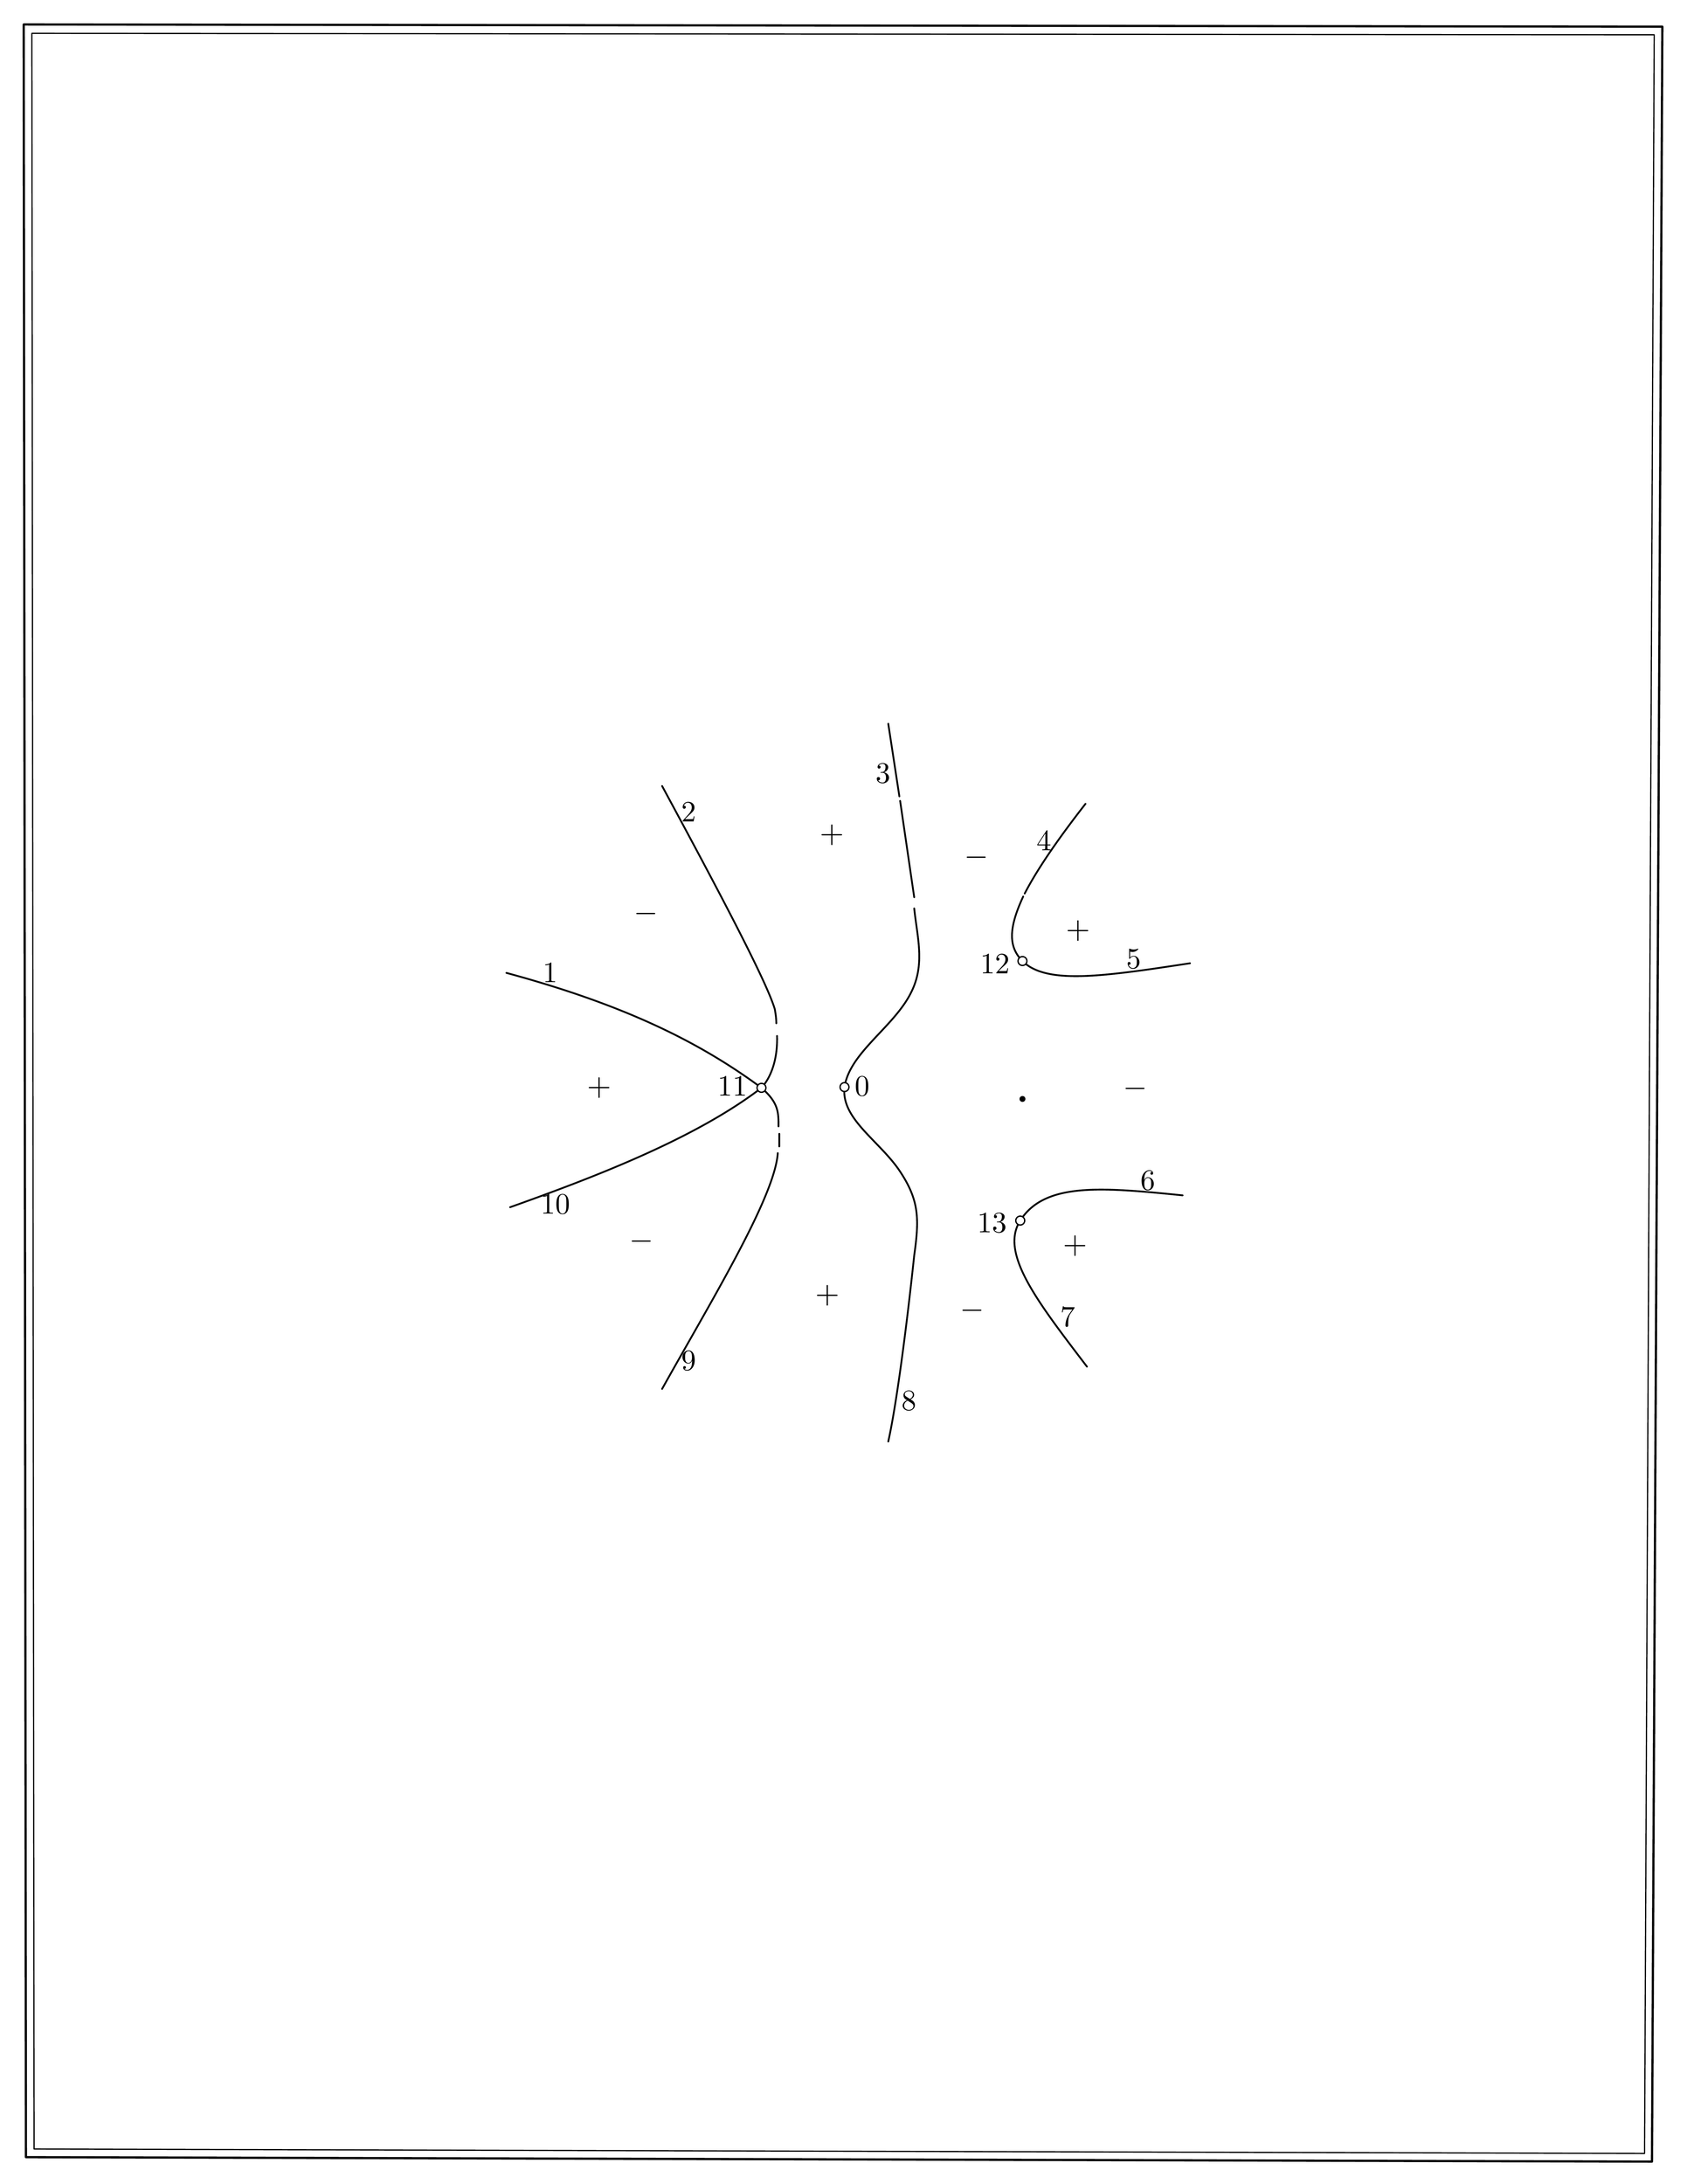
\begin{tikzpicture}[x=1bp,y=-1bp,line cap=round,line join=round]
\path[use as bounding box] (0,0) rectangle (2255,2925);
\begin{pgfinterruptboundingbox}
\draw[line width=3bp] (22,23) -- (2232,26) -- (2218,2905) -- (25,2899) -- cycle;
\draw[line width=1.6bp] (33,35) -- (2221,37) -- (2208,2894) -- (36,2888) -- cycle;
\draw[line width=2.4bp] (673,1302) .. controls (832,1345) and (933,1395) .. (1017,1457) .. controls (1040,1477) and (1040,1490) .. (1040,1509);
\draw[line width=2.4bp] (1041,1519) -- (1041,1536);
\draw[line width=2.4bp] (1039,1545) .. controls (1035,1604) and (950,1743) .. (883,1863);
\draw[line width=2.4bp] (883,1050) .. controls (944,1163) and (1023,1310) .. (1035,1351) .. controls (1036,1357) and (1037,1363) .. (1037,1370);
\draw[line width=2.4bp] (1038,1387) .. controls (1039,1422) and (1028,1445) .. (1017,1457) .. controls (927,1526) and (790,1578) .. (678,1618);
\draw[line width=2.4bp] (1188,966) -- (1203,1064);
\draw[line width=2.4bp] (1204,1070) -- (1223,1200);
\draw[line width=2.4bp] (1223,1215) .. controls (1227,1254) and (1238,1290) .. (1219,1328) .. controls (1196,1375) and (1136,1409) .. (1129,1456) .. controls (1124,1498) and (1174,1527) .. (1202,1567) .. controls (1230,1608) and (1230,1633) .. (1223,1683) .. controls (1214,1768) and (1200,1880) .. (1188,1934);
\draw[line width=2.4bp] (1454,1074) .. controls (1415,1124) and (1388,1164) .. (1372,1195);
\draw[line width=2.4bp] (1370,1199) .. controls (1350,1242) and (1350,1267) .. (1369,1286) .. controls (1401,1318) and (1477,1307) .. (1595,1289);
\draw[line width=2.4bp] (1585,1602) .. controls (1476,1591) and (1399,1584) .. (1366,1636) .. controls (1338,1680) and (1389,1745) .. (1456,1833);
\draw[fill=white,line width=1.8bp] (1017,1457) circle[radius=6bp];
\draw[fill=white,line width=1.8bp] (1129,1456) circle[radius=6bp];
\draw[fill=white,line width=1.8bp] (1369,1286) circle[radius=6bp];
\draw[fill=white,line width=1.8bp] (1366,1636) circle[radius=6bp];
\fill (1369,1472) circle[radius=4bp];
\node[inner sep=0pt,outer sep=0pt,rotate=0] at (732,1302) {\scalebox{4.0}{\ensuremath{1}}};
\node[inner sep=0pt,outer sep=0pt,rotate=0] at (919,1085) {\scalebox{4.0}{\ensuremath{2}}};
\node[inner sep=0pt,outer sep=0pt,rotate=0] at (1181,1033) {\scalebox{4.0}{\ensuremath{3}}};
\node[inner sep=0pt,outer sep=0pt,rotate=0] at (1398,1124) {\scalebox{4.0}{\ensuremath{4}}};
\node[inner sep=0pt,outer sep=0pt,rotate=0] at (1519,1283) {\scalebox{4.0}{\ensuremath{5}}};
\node[inner sep=0pt,outer sep=0pt,rotate=0] at (1538,1582) {\scalebox{4.0}{\ensuremath{6}}};
\node[inner sep=0pt,outer sep=0pt,rotate=0] at (1430,1766) {\scalebox{4.0}{\ensuremath{7}}};
\node[inner sep=0pt,outer sep=0pt,rotate=0] at (1216,1879) {\scalebox{4.0}{\ensuremath{8}}};
\node[inner sep=0pt,outer sep=0pt,rotate=0] at (919,1825) {\scalebox{4.0}{\ensuremath{9}}};
\node[inner sep=0pt,outer sep=0pt,rotate=0] at (739,1614) {\scalebox{4.0}{\ensuremath{10}}};
\node[inner sep=0pt,outer sep=0pt,rotate=0] at (978,1455) {\scalebox{4.0}{\ensuremath{11}}};
\node[inner sep=0pt,outer sep=0pt,rotate=0] at (1153,1455) {\scalebox{4.0}{\ensuremath{0}}};
\node[inner sep=0pt,outer sep=0pt,rotate=0] at (1332,1290) {\scalebox{4.0}{\ensuremath{12}}};
\node[inner sep=0pt,outer sep=0pt,rotate=0] at (1328,1639) {\scalebox{4.0}{\ensuremath{13}}};
\node[inner sep=0pt,outer sep=0pt,rotate=0] at (1112,1116) {\scalebox{4.2}{\ensuremath{+}}};
\node[inner sep=0pt,outer sep=0pt,rotate=0] at (798,1457) {\scalebox{4.2}{\ensuremath{+}}};
\node[inner sep=0pt,outer sep=0pt,rotate=0] at (1444,1245) {\scalebox{4.2}{\ensuremath{+}}};
\node[inner sep=0pt,outer sep=0pt,rotate=0] at (1440,1670) {\scalebox{4.2}{\ensuremath{+}}};
\node[inner sep=0pt,outer sep=0pt,rotate=0] at (1106,1737) {\scalebox{4.2}{\ensuremath{+}}};
\node[inner sep=0pt,outer sep=0pt,rotate=0] at (861,1222) {\scalebox{4.2}{\ensuremath{-}}};
\node[inner sep=0pt,outer sep=0pt,rotate=0] at (1307,1146) {\scalebox{4.2}{\ensuremath{-}}};
\node[inner sep=0pt,outer sep=0pt,rotate=0] at (1521,1458) {\scalebox{4.2}{\ensuremath{-}}};
\node[inner sep=0pt,outer sep=0pt,rotate=0] at (1301,1757) {\scalebox{4.2}{\ensuremath{-}}};
\node[inner sep=0pt,outer sep=0pt,rotate=0] at (855,1664) {\scalebox{4.2}{\ensuremath{-}}};
\end{pgfinterruptboundingbox}
\end{tikzpicture}
